\section{Introduction}
In this chapter we consider similar projects that have been done and how they relate to the project development and execution in relation to our project. We also look at their short coming so that we can improve those areas in our project

\subsection{Makerere University Automated Payment System}
This is the existing system in place in our area of study. The project was commenced in 2014 by Makerere University in collaboration with Kenya Airport Parking Services . From our interviews with the owners of the system, we learned that he system costs approximately 1.5 billion shillings to set up, and consists of a ticketing machine that issues tickets to motorists that they are then required to present at one of the various payment points within the university. Some of the chellenges in this system include:
\begin{itemize}
    \item Frequent malfunction of the ticketing machines
    \item Fraud by the system employees
    \item Difficulty in locating a payment point for motorists
    \item Hefty fines for lost tickets as motorists who misplace their tickets are required to pay a fine of 50,000 Uganda Shillings
    \item Inconvenience, inefficiency, and revenue loss for both the system’s managers and motorists.
\end{itemize}

\subsection{Uganda National Roads Authority Express Highway}
\begin{figure}
    \begin{center}
        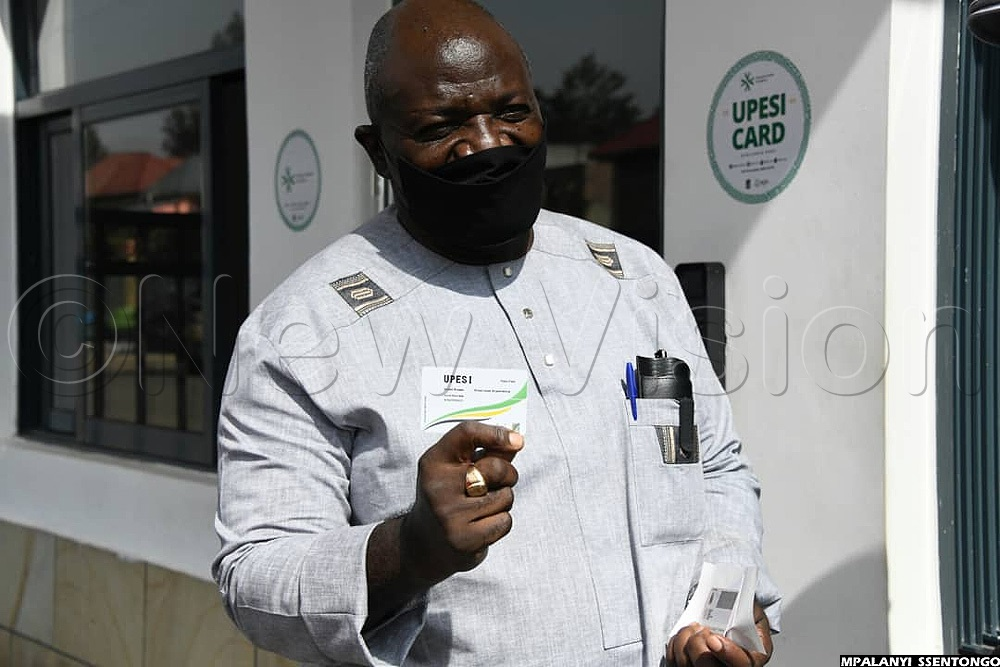
\includegraphics[scale = 0.3]{images/katus}
        \caption{Gen. Katumba Wamala showing an UPESI payment card on the launch of the Entebbe Express Highway}
    \end{center}
\end{figure}
The Uganda National Roads Authority in 2022 launched the Kampala Entebbe Express Highway, a Ugandan government project worth approximately 450 million dollars developed to help ease transport flow in Kampala city. Access to the highway is via the toll gates where motorists can make both cash and digital cashless payments. For cashless payments, motorists use an UPESI card.\cite{unra_news_2022}. A motorist purchases an UPESI card that they then load a given amount of money and upon arrival at the toll gate, they swipe the card. The fee is then deducted from the card and the motorist is then granted access.

The main gap with the approach is motorists often resort to only using the cash payments that result in delays and other issues because they find it easier than purchasing an UPESI card. Additionally the process of loading money onto the card is unnecessarily long. Fine for losing card.

\subsection{ParkMobile}
Parkmobile is a leading mobile application launched in 2009 in the United States of America that allows motorists to find and pay for parking on their phone, and is currently used in approximately used in three thousand lcoations in North America. It also has over 43 million users and processed over 113 million parking transactions in 2022.
Parkmobile offers various features and benefits for its users, such as making prepayments and reserving parking points at any given location. It also offers a rewards program that allows users to earn points for every parking transaction and redeem them for discounts or free parking. Parkmobile also supports Google and Apple Pay for a faster and more secure payment process. \cite{parkmobile_2022}
The projeect has had good traction since it was launched and in 2022 it generated $9.1 million in revenue , with an average revenue per employee of $52,906. Parkmobile was acquired by EasyPark Group, a Swedish company that provides smart parking and mobility solutions, in June 2021.

Unfortunately to the best of our knowledge, ParkMobile or any other application of this nature are not available in Uganda thus the need for a local contextualised solution

\subsection{Use of GPS Software and Cell Towers}
Research on how this can be leveraged in easing toll fee payment has been done by others. In 2020, Danang Dismantoro, Istas Pratomo and Surya Sumpeno also proposed a mobile application that allowed payment of these fees via GPS software\cite{el-rabbany_introduction_2002,dismantoro_minimizing_2020}. The system was tested through simulations in Vissim software \cite{ptv_vissim_traffic_2022}, which they believe was able to simulate the real world condition at tollgates. Cell phone towers and GPS technology are used to identify the motorist’ s location and if the motorist happens to be within the toll’s gate vicinity, the money is automatically deducted from their personal account.

\subsubsection{Research Gaps}
\begin{itemize}
    \item No physical implementation of this system was realised
    \item The researchers acknowledge the need for a deeper feasibility study and the fact as it has some shortcomings.
    \item Some scenarios are unaccounted for such as if one is near a cell tower but does not necessarily intend to access the tollgate,they’ll have their money deducted even without actually using the gate.
\end{itemize}

\subsection{Use of RFID sensors}
An RFID system has two main components:
\begin{itemize}
    \item A transponder: This is the tag that holds information, found on the object to be identified
    \item A reader/interrogator: This device is able to capture data from the tag.It has a radio frequency module,  control unit and coupling element for linking to the transponder. Additionally, an interface is added to pass on data captured from the transponder to a different system
\end{itemize}


Sabbir Ahmed et al in 2019 also proposed a similar solution.Their proposed system would simplify toll payment through use of RFID tags placed on digitised license plates of all vehicles.Once the tag is scanned, and the motorist has a sufficient balance on their account, the vehicle is granted access\cite{ahmed_automated_2019}.


Another study by Etqad Khan et al. in 2018 proposed a system similar to ours that would ease payment of toll fees using RFID tag that would be linked to motorists' personal accounts where would have a mobile e-wallet on which a given amount would be saved.The system also provides a mobile application to view their past payments\cite{khan_automated_2018}.

\begin{figure}
    \begin{center}
        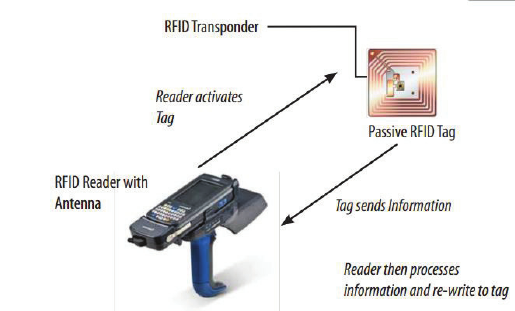
\includegraphics[scale = 0.3]{images/rfid-pic}
        \caption{Components of an RFID system}
    \end{center}
\end{figure}

\subsubsection{Research Gap}
These two identified studies are constrained in our project scope’s context, because:
\begin{itemize}
    \item It would first off require digitisation of all vehicle license plate, an endeavour that has not yet been taken on by the government of Uganda.
    \item Long range RFID tags and scanners are costly to purchase which would be needed in this use case are costly ,and would thus the need for a low-cost solution that’s accessible to majority of the motorists.
\end{itemize}



\clearpage


\section{Our Contribution}
Alot of work has been done by other researchers to address the issue of tollgate queues. Many of these solutions leverage RFID technology as an alternative to the physical cash payments. This would however require purchasing costly scanners and tags, thus the need for a similar but cheaper solution.
The biggest benefits to our proposed system:
\begin{itemize}
    \item Developing a low-cost and context-specific solution for cashless parking payment using local popular payment platforms such as MTN mobile money
    \item Designing and implementing a mobile app and an embedded microcontroller that interact using QR codes to facilitate parking access and payment
    \item Evaluating the performance and usability of the system and comparing it with the current system of ticketing and payment
    \item Examining the benefits and challenges of the system, such as security, scalability, and user acceptance
    \item Providing insights and recommendations for improving parking management in the university context and in developing countries in general
\end{itemize}

\begin{figure}
    \begin{center}
        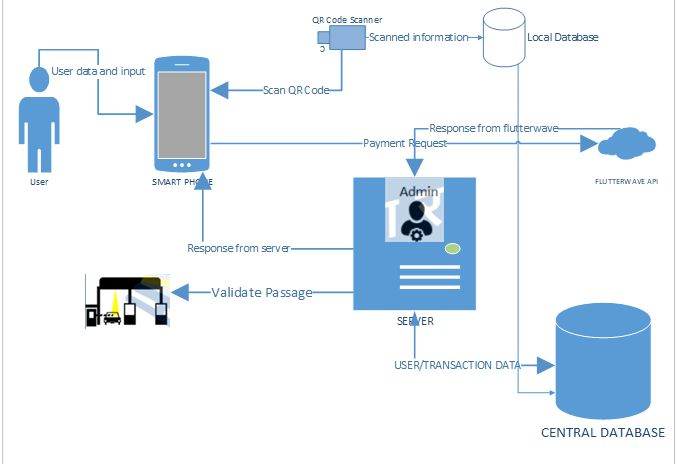
\includegraphics[scale = 0.6]{images/etolssys}
        \caption{System Architecture Diagram for the proposed solution }
    \end{center}
\end{figure}